% Options for packages loaded elsewhere
\PassOptionsToPackage{unicode}{hyperref}
\PassOptionsToPackage{hyphens}{url}
%
\documentclass[
  12pt,
]{article}
\usepackage{amsmath,amssymb}
\usepackage{iftex}
\ifPDFTeX
  \usepackage[T1]{fontenc}
  \usepackage[utf8]{inputenc}
  \usepackage{textcomp} % provide euro and other symbols
\else % if luatex or xetex
  \usepackage{unicode-math} % this also loads fontspec
  \defaultfontfeatures{Scale=MatchLowercase}
  \defaultfontfeatures[\rmfamily]{Ligatures=TeX,Scale=1}
\fi
\usepackage{lmodern}
\ifPDFTeX\else
  % xetex/luatex font selection
\fi
% Use upquote if available, for straight quotes in verbatim environments
\IfFileExists{upquote.sty}{\usepackage{upquote}}{}
\IfFileExists{microtype.sty}{% use microtype if available
  \usepackage[]{microtype}
  \UseMicrotypeSet[protrusion]{basicmath} % disable protrusion for tt fonts
}{}
\makeatletter
\@ifundefined{KOMAClassName}{% if non-KOMA class
  \IfFileExists{parskip.sty}{%
    \usepackage{parskip}
  }{% else
    \setlength{\parindent}{0pt}
    \setlength{\parskip}{6pt plus 2pt minus 1pt}}
}{% if KOMA class
  \KOMAoptions{parskip=half}}
\makeatother
\usepackage{xcolor}
\usepackage[margin=1in]{geometry}
\usepackage{graphicx}
\makeatletter
\def\maxwidth{\ifdim\Gin@nat@width>\linewidth\linewidth\else\Gin@nat@width\fi}
\def\maxheight{\ifdim\Gin@nat@height>\textheight\textheight\else\Gin@nat@height\fi}
\makeatother
% Scale images if necessary, so that they will not overflow the page
% margins by default, and it is still possible to overwrite the defaults
% using explicit options in \includegraphics[width, height, ...]{}
\setkeys{Gin}{width=\maxwidth,height=\maxheight,keepaspectratio}
% Set default figure placement to htbp
\makeatletter
\def\fps@figure{htbp}
\makeatother
\setlength{\emergencystretch}{3em} % prevent overfull lines
\providecommand{\tightlist}{%
  \setlength{\itemsep}{0pt}\setlength{\parskip}{0pt}}
\setcounter{secnumdepth}{-\maxdimen} % remove section numbering
\newlength{\cslhangindent}
\setlength{\cslhangindent}{1.5em}
\newlength{\csllabelwidth}
\setlength{\csllabelwidth}{3em}
\newlength{\cslentryspacingunit} % times entry-spacing
\setlength{\cslentryspacingunit}{\parskip}
\newenvironment{CSLReferences}[2] % #1 hanging-ident, #2 entry spacing
 {% don't indent paragraphs
  \setlength{\parindent}{0pt}
  % turn on hanging indent if param 1 is 1
  \ifodd #1
  \let\oldpar\par
  \def\par{\hangindent=\cslhangindent\oldpar}
  \fi
  % set entry spacing
  \setlength{\parskip}{#2\cslentryspacingunit}
 }%
 {}
\usepackage{calc}
\newcommand{\CSLBlock}[1]{#1\hfill\break}
\newcommand{\CSLLeftMargin}[1]{\parbox[t]{\csllabelwidth}{#1}}
\newcommand{\CSLRightInline}[1]{\parbox[t]{\linewidth - \csllabelwidth}{#1}\break}
\newcommand{\CSLIndent}[1]{\hspace{\cslhangindent}#1}
\usepackage{setspace}\doublespacing
\usepackage{amsmath}
\usepackage{lineno}
\linenumbers
\usepackage{fontspec}
\setmainfont{Times New Roman}
\usepackage{placeins}
\renewcommand{\figurename}{Figure S}
\makeatletter
\renewcommand{\fnum@figure}{\figurename~\thefigure}
\makeatother
\ifLuaTeX
  \usepackage{selnolig}  % disable illegal ligatures
\fi
\IfFileExists{bookmark.sty}{\usepackage{bookmark}}{\usepackage{hyperref}}
\IfFileExists{xurl.sty}{\usepackage{xurl}}{} % add URL line breaks if available
\urlstyle{same}
\hypersetup{
  pdftitle={Extended Data: Size spectra in freshwater streams are consistent across temperature and resource supply},
  hidelinks,
  pdfcreator={LaTeX via pandoc}}

\title{Extended Data: Size spectra in freshwater streams are consistent
across temperature and resource supply}
\author{}
\date{\vspace{-2.5em}}

\begin{document}
\maketitle

\emph{Vojsava Gjoni}\textsuperscript{1}, \emph{Justin P.F.
Pomeranz}\textsuperscript{2}, \emph{James R. Junker}\textsuperscript{3},
\emph{Jeff Wesner}\textsuperscript{1}

\textsuperscript{1}University of South Dakota, Department of Biology,
Vermillion, SD 57069

\textsuperscript{2}Colorado Mesa University, Department of Physical and
Environmental Sciences, Grand Junction, CO 81501

\textsuperscript{3}University of North Texas, Department of Biological
Sciences, Denton, TX 76203

\hypertarget{model-checking}{%
\subsection{Model Checking}\label{model-checking}}

We examined model fit using Bayesian R\(^2\) (Gelman et al. 2019) ,
posterior predictive checks (Gabry et al. 2019), and Bayesian P-values
(Hobbs and Hooten 2015). Each of these measures summarize comparisons
between the raw data and data predicted from the posterior distribution
of the fitted model. To do this, we first needed to remove the
\(counts\) variable from the raw data. It contains the density of each
individual body size, which allows us to combine the fish and
macroinvertebrate data sets while accounting for the different
collection areas and relative abundances of each taxa (J. Wesner and
Pomeranz 2023). However, while the densities are included in the
likelihood when fitting the model, they are not included in the random
number generator for simulating data. Therefore, to remove them, we
re-sampled 5,000 individual body sizes with replacement from each of the
133 samples, weighting each sample by its density in no/m\(^2\) . This
generated a vector of individual body sizes, each with an implied
density of 1.

To simulate new data from the posterior, we first extracted the
posterior distribution of \(\lambda\) for each of the \(j =\) 133
samples using the \texttt{add\_epred\_draws()} function from the
\texttt{tidyabayes} package (Kay, n.d.). This function applies the
following:

\[
\lambda_j^k = g(\boldsymbol{ \theta}^k_j, \text{X}_j)
\]

where \(\lambda_j^k\) is the \(k^{\text{th}}\) posterior draw from
sample \(j\), derived from the linear equation containing the
\(k^{\text{th}}\) parameter values \(\boldsymbol {\theta}\) and data
\(\text{X}\) associated with sample \(j\). From the first 100 \(k\)
draws of each \(\lambda_j\), we simulated 5,000 individual body sizes
using the inverse cumulative density function J. S. Wesner et al. (2023)
via the \texttt{rparetocounts} function from the R package
\texttt{isdbayes} J. Wesner and Pomeranz (2023).

The end result is 5000 simulated individual body sizes from each of the
133 NEON samples. This allowed us to compare model fit at the sample
level. We also compared fits from the full model using the posterior
mean estimate of \(\lambda\). In other words, we simulated the full data
set rather than data sets for each sample \(j\).

To determine how well the model recaptures the raw data, we visually
compared the simulated data, \(y_{pred,j}\), and the raw re-sampled
data, \(y_j\) of each \(j\) sample. We also calculated the geometric
mean for each \(j\) prediction and raw data. We then calculated a
Bayesian P-value as the proportion of posterior draws for which the
geometric mean was greater than the raw value. Proportions
\textgreater0.1 or \textless0.9 are generally indicative of poor model
fit, indicating a mismatch in the \(ypred\) and \(y\) (Hobbs and Hooten
2015).

Finally, we calculated a Bayesian R\(^2\) using the formula given in
Gelman et al. (2019):

\[  R^2 = \frac{\text{V}_{ypred}}{\text{V}_{ypred} + \text{V}_{res}}, \]

where \(\text{V}_{ypred}\) is the variance of \(ypred\) and
\(\text{V}_{res}\) is the variance of the residuals \(ypred - y\). We
repeated this equation for each of 1,000 \(k\) draws from the posterior,
generating a distribution of \(R^2\).

\emph{Results}

The model had a Bayesian R\(^2\) of 0.47 \(\pm\) 0.02 (mean \(\pm\) sd),
indicating good fit explaining \textasciitilde47\% of the variance of
new data. Posterior predictive checks revealed generally good fit
(Figure ED1). First, the predictive distributions in Figure ED1
generally resemble the raw re-sampled distributions. This suggests that
the truncated Pareto is a reasonable likelihood for these data. However,
there are several clear discrepancies. For example, there is variation
in fit among sites, with MCDI and KING sites appearing strong, while
sites like GUIL and BLUE have more of their raw distributions in larger
body size ranges compared to the posterior predictive. These may
indicate either deviations from a power law at these sites due to
underlying mechanisms in the food web. Alternatively, they can indicate
an under sampling of either large or small individuals during field
collections, or a combination of the two. Our perspective is that the
truncated Pareto provides a reasonably good fit to the data overall.

Despite some variation among sites between \(y_{pred}\) and \(y\), there
is strong agreement in the geometric means (GM) across samples. Figure
ED2 shows the GM(\(y_{pred}\)) compared to the GM(\(y\)) across all 133
samples. The GM(\(y\)) is consistently within the 95\% credible
intervals of GM(\(y_{pred}\)) at each sample (Figure ED2). Moreover,
Bayesian P-values across all samples ranged from 0.13 to 0.84 with a
mean of 0.5 and sd of 0.14, again indicating good overall model fit.

\hypertarget{references}{%
\section{References}\label{references}}

\hypertarget{refs}{}
\begin{CSLReferences}{1}{0}
\leavevmode\vadjust pre{\hypertarget{ref-gabry2019}{}}%
Gabry, J., D. Simpson, A. Vehtari, M. Betancourt, and A. Gelman. 2019.
{``Visualization in Bayesian Workflow.''} \emph{J. R. Stat. Soc. A.
Stat} 182: 389402.

\leavevmode\vadjust pre{\hypertarget{ref-gelman2019r}{}}%
Gelman, Andrew, Ben Goodrich, Jonah Gabry, and Aki Vehtari. 2019.
{``R-Squared for Bayesian Regression Models.''} \emph{The American
Statistician}.

\leavevmode\vadjust pre{\hypertarget{ref-hobbs2015}{}}%
Hobbs, N. Thompson, and Mevin B. Hooten. 2015. \emph{Bayesian Models:
{A} Statistical Primer for Ecologists}. {Princeton University Press}.
\url{https://doi.org/10.23943/princeton/9780691159287.001.0001}.

\leavevmode\vadjust pre{\hypertarget{ref-kay_tidy}{}}%
Kay, Matthew. n.d. \emph{{tidybayes}: Tidy Data and Geoms for {Bayesian}
Models}. \url{https://doi.org/10.5281/zenodo.1308151}.

\leavevmode\vadjust pre{\hypertarget{ref-wesner2023bayesian}{}}%
Wesner, Jeff S, Justin PF Pomeranz, James R Junker, and Vojsava Gjoni.
2023. {``Bayesian Hierarchical Modeling of Size Spectra.''}
\emph{bioRxiv}, 2023--02.

\leavevmode\vadjust pre{\hypertarget{ref-wesner2023isdbayes}{}}%
Wesner, Jeff, and Justin Pomeranz. 2023. \emph{Isdbayes: Bayesian
Hierarchical Modeling of Power Laws Using Brms}.

\end{CSLReferences}

\newpage

\begin{figure}
\includegraphics[width=1\linewidth]{../plots/post_pred_i} \caption{Posterior predictive check showing the distribution of the raw re-sampled (y) data compared to 10 draws from teh posterior predictive distribution. The results are visualized at the site level here, but the distributions reflect simulations from each individual sample within a site.}\label{fig:unnamed-chunk-1}
\end{figure}

\newpage

\begin{figure}
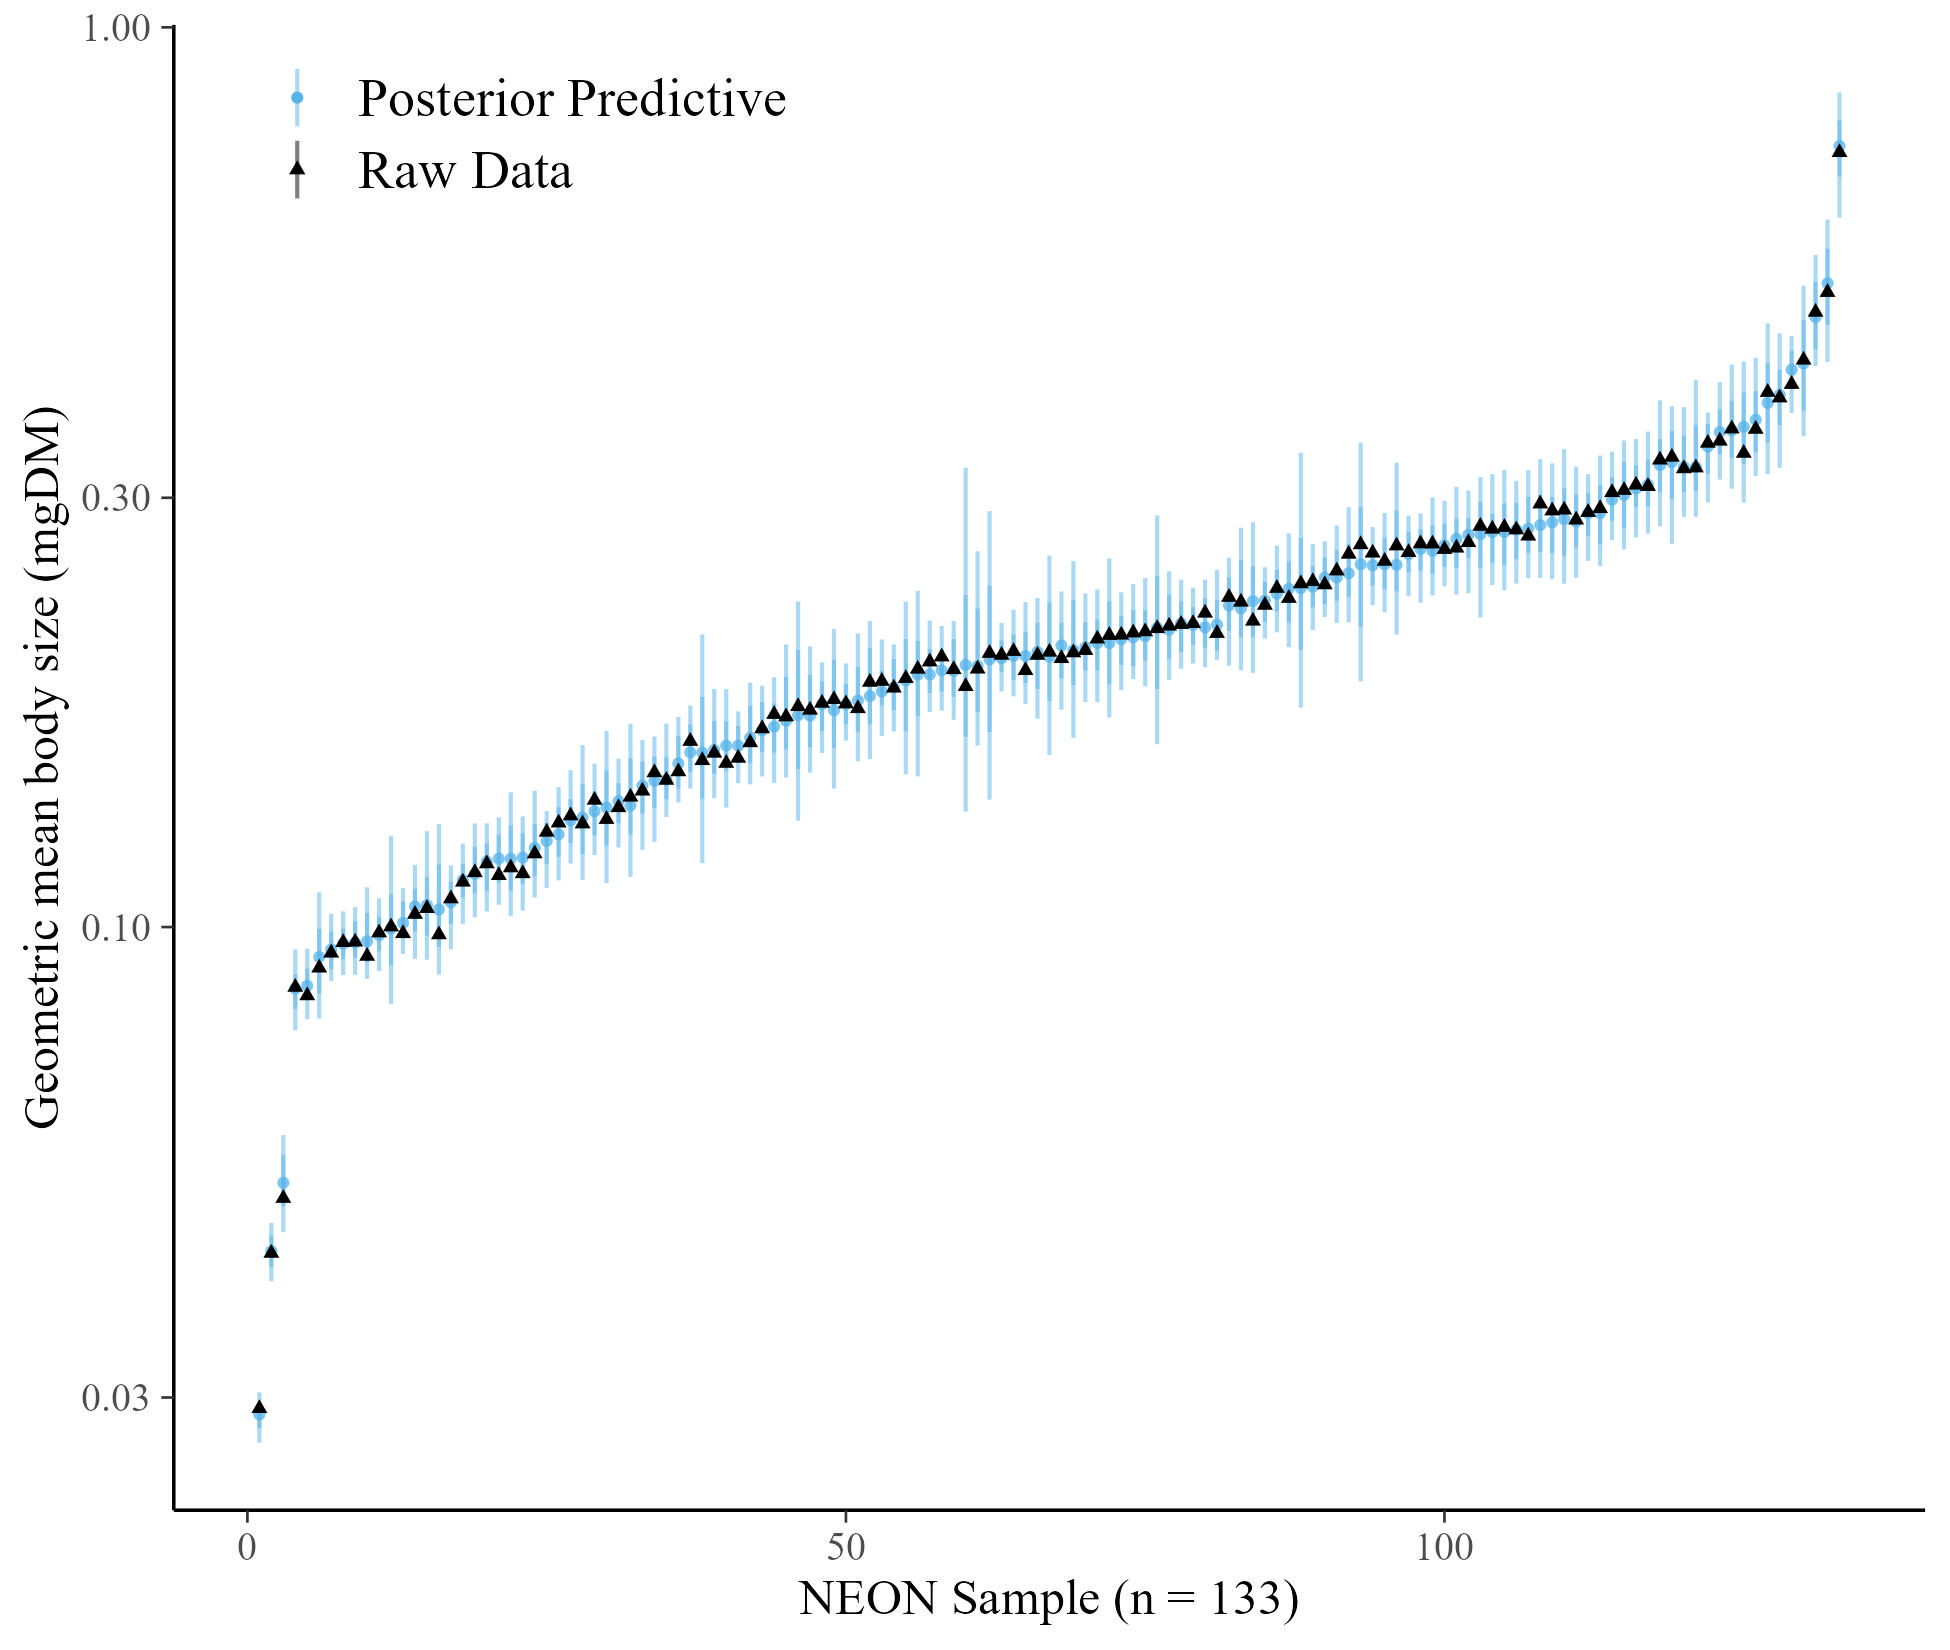
\includegraphics[width=1\linewidth]{../plots/post_pred_gm} \caption{Posterior predictive check showing the geometric mean body size calculated from the raw re-sampled data (black triangle) compared to the geometric mean calculatd from the posterior predictive distribution (blue dot and line). The blue dot and line represent the median and 95\% quantiles from 100 draws of the posterior distribution}\label{fig:unnamed-chunk-2}
\end{figure}

\end{document}
